\clearpage

\begin{tcolorbox}	
\begin{tabular}{p{2.75cm} p{0.2cm} p{10.5cm}} 	
\textbf{Student Name}  &:& Tiago Esteves\\
\textbf{Starting Date} &:& October 03, 2017\\
\textbf{Goal}          &:& Implement the dimensioning of optical networks in the translucent transport mode.
\end{tabular}
\end{tcolorbox}

\section{Transparent with 1+1 Protection}
In this case study we focus on the transparent case with 1 + 1 protection. \\
In this mode of transport, the information travels in a route defined through optical channels between origin and destination nodes always in the optical domain and, consequently, physical topology and logical topology are different.
An advantage of this mode of transport is the possibility of transporting express traffic.
An disadvantage is that the capacity utilization of the optical channels is worse than in the opaque mode of transport due to grooming only customer signs with the same endpoints.

\subsection{Physical Network Topology}

\subsubsection{Reference Network}
In the figure below we can see that our reference network consists of 6 nodes and 8 Bidirectional links.
The average length of the links was chosen so that the following calculations are more simplistic.

\begin{figure}[h!]
\centering
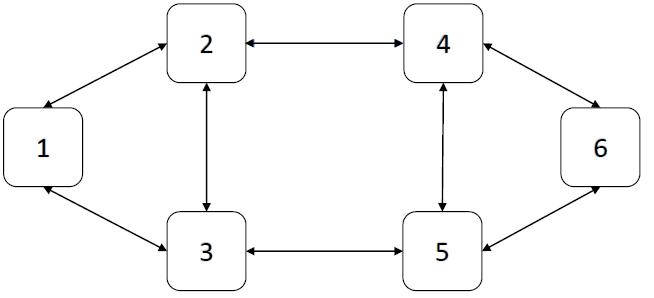
\includegraphics[width=\textwidth]{RedeTeste}
\caption{Physical Topology of the Reference Network.}
\end{figure}

As we can see from table \ref{table:3}, to do all the calculations necessary for this project, let us know the value of the traffic used. This value is defined depending on the scenario used, as we can see:

\begin{itemize}
  \item Low Traffic: \textbf{0.5 TBits/s}
  \item High Traffic: \textbf{5 TBits/s}
\end{itemize}

\begin{table}[h!]
The following table shows the values of the variables associated with this network.\vspace{10pt}
\centering
\begin{tabular}{|| c | c | c||}
 \hline
 Constant & Description & Value \\
 \hline\hline
 N & Number of Nodes & 6 \\
 L & Number of Bidirectional Links & 8 \\
 <$\delta$> & Node out-degree & 2,667 \\
 <len> & Mean Link Length (km) & 500 \\
 <h> & Mean Number of Hops,for Working Paths & 1,533 \\
 <h'> & Mean Number of Hops,for Backup Paths & 2,467 \\
 \hline
\end{tabular}
\caption{Table of reference network values}
\label{table:3}
\end{table}



\subsubsection{Realistic Network}
The real network chosen for this work is the EON (European Optical Network).
The way the nodes are arranged geographically can be seen from the following figure.

\begin{figure}[h!]
\centering
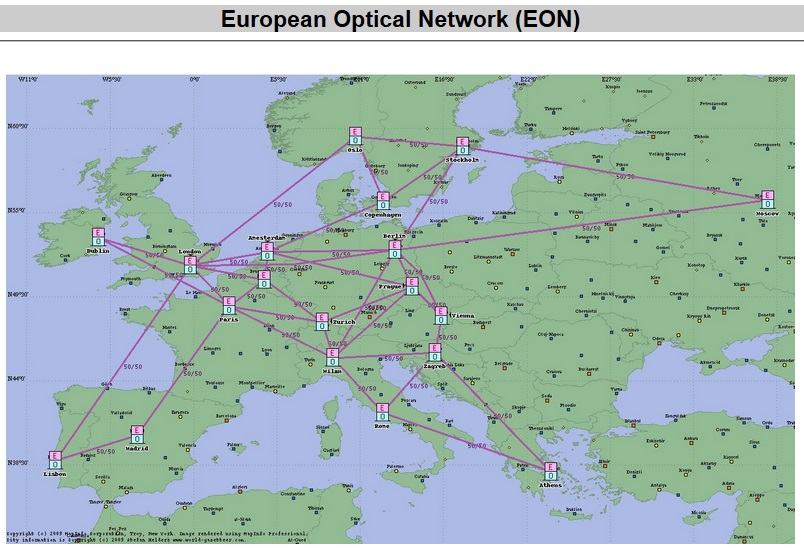
\includegraphics[width=\textwidth]{EON_Rede_Realista}
\caption{Physical Topology of the Realistic Network.}
\end{figure}

\begin{table}[h!]
The table \ref{table:4} shows the values of the variables associated with this network.\vspace{10pt}
\centering
\begin{tabular}{|| c | c | c||}
 \hline
 Constant & Description & Value \\
 \hline\hline
 N & Number of Nodes & 19 \\
 L & Number of Bidirectional Links & 37 \\
 <$\delta$> & Node out-degree & 3,89 \\
 <len> & Mean Link Length (km) & 753,76 \\
 <h> & Mean Number of Hops,for Working Paths & 2,3 \\
 <h'> & Mean Number of Hops,for Backup Paths & 3,2 \\
 \hline
\end{tabular}
\caption{Table of realistic network values}
\label{table:4}
\end{table}

\vspace{10pt}

Again, to make all the necessary calculations, only the value of the traffic used is missing. This value is set depending on the scenario used, as we can see:

\begin{itemize}
  \item Low Traffic: \textbf{2 TBits/s}
  \item High Traffic: \textbf{20 TBits/s}
\end{itemize}

\subsection{Dimensioning using ILP}
\vspace{10pt}
\subsubsection{ILP Models} \label{ILP_models_Transp}

Again, for a better understanding of the functions and variables used in the ILP, a table \ref{description_transp} will be created with all the variables and their description. \\

\begin{table}[h!]
\centering
\begin{tabular}{|| c | c||}
 \hline
 Variables & Description \\
 \hline\hline
 $($ i,j $)$ & Origin node, i and destination node, j of a Link \\
 $($ o,d $)$ & Origin node, o and destination node, d of a Demand \\
 f & Number of 100 Gbit/s optical channels (number of flows) \\
 W & Number of optical channels \\
 x & I'm not sure what this variable means \\
 G & Network topology in form of Adjacency matrix \\
 \hline
\end{tabular}
\caption{Table with description of variables}
\label{description_transp}
\end{table}

\vspace{20pt}

The optimization model suggested for transparent transport mode with dedicated path protection intends to minimize the total number of flows crossing link (i, j) for all demand pairs (o, d). The mathematical model described below also minimizes the total number of optical channels between each demand end nodes $W_{od}$, instead of minimizing the number of optical link-by-link channels as in the previous model.

\newpage

\begin{equation}
minimize    \sum_{(i,j)} \sum_{(o,d)} f_{ij}^{od} + \sum_{(o,d)} W_{od}
\label{ILPTransp}
\end{equation}

$subject$ $to$
\begin{equation}
\sum_{j\textbackslash \{o\}} f_{ij}^{od} = 2  \qquad \qquad \qquad \qquad \qquad \qquad \qquad \qquad \qquad \qquad
\forall(o,d) : o < d, \forall i: i = o
\label{ILPTransp1}
\end{equation}

\begin{equation}
\sum_{j\textbackslash \{o\}} f_{ij}^{od} = \sum_{j\ \{d\}} f_{ji}^{od}   \qquad \qquad \qquad \qquad \qquad \qquad \qquad \qquad
\forall(o,d) : o < d, \forall i: i \neq o,d
\label{ILPTransp2}
\end{equation}

\begin{equation}
\sum_{j\textbackslash \{d\}} f_{ji}^{od} = 2  \qquad \qquad \qquad \qquad \qquad \qquad \qquad \qquad \qquad \qquad
\forall(o,d) : o < d, \forall i: i = d
\label{ILPTransp3}
\end{equation}

\begin{equation}
\sum_{(o,d):o<d} \left(f_{ij}^{od} + f_{ji}^{od}\right) x W_{od} \leq 80 G_{ij} \qquad \qquad \qquad \qquad \qquad \qquad \qquad \qquad
\forall(i,j) : i < j
\label{ILPTransp4}
\end{equation}

\begin{equation}
f_{ij}^{od} , f_{ji}^{od} \in \{0,2\}   \qquad \qquad \qquad \qquad \qquad \qquad \qquad \qquad \qquad
\forall(i,j) : i < j, \forall(o,d) : o < d
\label{ILPTransp5}
\end{equation}

\begin{equation}
W_{od} \in \mathbb{N}  \qquad \qquad \qquad \qquad \qquad \qquad \qquad \qquad \qquad \qquad \qquad \qquad \qquad
\forall(o,d) : o < d
\label{ILPTransp6}
\end{equation}

\vspace{10pt}

The objective function, to be minimized, is the expression \ref{ILPTransp}. The flow conservation is performed by equations \ref{ILPTransp1}, \ref{ILPTransp2} and \ref{ILPTransp3} and share the same mathematical description of opaque model. The inequality \ref{ILPTransp4} answers capacity constraint problem. Then, total flows times the traffic of the demands must be less or equal to the capacity of network links. The grooming of this model can be done before routing since the traffic is aggregated just for demands between the same nodes, thus not depending on the routes. Last two constraints define the total number of flows must be zero if there is no demand, or two for a demand with traffic protection, and the number of optical channels must be a counting number.

\newpage
\subsubsection{ILP Results}

In this initial phase the results will be presented using ILP to calculate the CAPEX of the reference network.

The value of the CAPEX of the network will be calculated based on the costs of the equipment present in the table below.
\begin{table}[h!]
\centering
\begin{tabular}{|| c | c||}
 \hline
 Equipment & Cost \\
 \hline\hline
 OLT without transponders & 15000 \euro \\
 Transponder & 5000 \euro/Gb \\
 Optical Amplifier & 4000 \euro \\
 EXC & 10000 \euro \\
 OXC & 20000 \euro \\
 EXC Port & 1000 \euro /Gb/s\\
 OXC Port & 2500 \euro /porto \\
 \hline
\end{tabular}
\caption{Table with costs}
\label{table_cost2}
\end{table}
In addition to the equipment costs, we will also use the parameter "span", which in this case will have a value of 100.
Because this value is used to calculate the number of optical amplifiers required in the network using Equation \ref{amplifiersTransp}.

\begin{equation}
N^R = \sum\limits_{l=1}^L\left(\left\lceil\frac{len_l}{span}\right\rceil-1\right)
\label{amplifiersTransp}
\end{equation} \\

To know the value of CAPEX it is necessary to know the value of the cost of the links and the cost of the nodes.

To calculate the cost of the nodes, the sum of the costs of the optical and electrical node is made. For this case the optical cost is given by equation \ref{opticalCost} and the electrical cost by the equation \ref{electricalCostTransp}.


\begin{equation}
C_{oxc} = \left(\gamma_{o0} \times N \right) + \gamma_{o1} \times  \left(P_{LINE} + P_{ADD}\right)
\label{opticalCost}
\end{equation}	
	
\begin{itemize}
\item{$C_{oxc}$		$\rightarrow$	Optical Ports Cost}
\item{$\gamma_{o0}$	$\rightarrow$	OXC cost in Euros}
\item{$\gamma_{o1}$	$\rightarrow$	OXC port cost in Euros}
\item{$P_{TRIB}	$	$\rightarrow$	Number of tributary ports}
\item{$P_{ADD} $	$\rightarrow$	Number of adding ports}
\end{itemize}

\begin{equation}
C_{exc} = \left(\gamma_{e0}\times N\right) + \gamma_{e1} \times \left(2 \times T_1 \right)		\label{electricalCostTransp}
\end{equation}

\vspace{10pt}

To calculate the cost of the Links we will use the equation \ref{linkCostsTransp}.

\begin{equation}
C_L = \left(\gamma_0^{OLT} \times L\right) + \left(\gamma_1^{OLT} \times \tau \times W\right) + \left(N^R \times c^R\right)
\label{linkCostsTransp}
\end{equation} \\
	
To perform the calculations using the implementation of the models described in section \ref{ILP_models_Transp} it is necessary to use a mathematical software tool. For this we will use MATLAB which is ideal for dealing with linear programming problems and can call the LPsolve through an external interface. \\

Using the values calculated through MatLab as well as the values indicated in table \ref{table:3} or table \ref{table:4} (depending on the scenario used) and table \ref{table_cost2} we can finally calculate the CAPEX value using equations \ref{electricalCostTransp}, \ref{opticalCost} and \ref{linkCostsTransp} for the various situations mentioned.\\


\textbf{Scenario 1: Test Network Low Traffic} \label{Scenario1_transp} \\

$C_L$ = \textbf{44 336 000\euro}

$C_N$ = $C_{oxc}$ + $C_{exc}$ = \textbf{2 515 000\euro}

$CAPEX$ = 44 336 000 + 2 515 000 = \textbf{46 851 000\euro}\\

\textbf{Scenario 2: Test Network High Traffic} \label{Scenario2_transp} \\

$C_L$ = \textbf{391 336 000\euro}

$C_N$ = $C_{oxc}$ + $C_{exc}$ = \textbf{21 445 000 \euro}

$CAPEX$ = 391 336 000 + 21 445 000 = \textbf{412 781 000 \euro}\\

\textbf{Scenario 3: Realistic Network Low Traffic} \label{Scenario3_transp} \\

$C_L$ = \textbf{\euro}

$C_N$ = $C_{exc}$ = \textbf{\euro}

$CAPEX$ =  +  = \textbf{\euro}\\

\textbf{Scenario 4: Realistic Network High Traffic} \label{Scenario4_transp} \\

$C_L$ = \textbf{\euro}

$C_N$ = $C_{exc}$ = \textbf{ \euro}

$CAPEX$ =  +  = \textbf{ \euro}\\


\subsection{Dimensioning using Heuristics}

\subsubsection{Heuristics Models}

\subsubsection{Heuristics Results}

\subsection{Analysis and comparison of results} 